\section{Exact-law validation and the deterministic certifiability phase map}
\label{sec:exact_phase}

Before benchmarking rough Bergomi, for which no closed-form price exists, we validate \RoughCertSPX{} against models with exact Fourier prices (Experiment~E1) and then test the full-determinism hypothesis across parameter space (Experiment~E2).

\subsection{Experiment E1: exact-law validation with correlated volatility}
\label{sec:e1}

We test the conditional Black--Scholes engine and the exact-bridge envelopes on three models with Fourier prices (\emph{exact-identity+quadrature}) at seven strikes $K\in\{0.85,\allowbreak 0.90,\allowbreak 0.95,\allowbreak 1.00,\allowbreak 1.05,\allowbreak 1.10,\allowbreak 1.15\}$, maturity $T=0.5$ and correlation $\rho=-0.7$:
\begin{enumerate}[1.]
  \item \emph{Correlated Heston \citep{Heston1993}} ($H=1/2$, $v_0=\theta=0.04$, $\kappa=2.0$, $\sigma_v=0.4$): the Little Heston Trap form \citep{AlbrecherMayerSchoutensTistaert2007} with \citet{Lewis2001} quadrature gives an ATM implied volatility of $\EOneHestonATMIV\%$; its martingale error is $\EOneHestonMart$ because the characteristic function equals one at $u=-\mathrm{i}$ identically.
  \item \emph{Classical correlated Stein--Stein \citep{SteinStein1991}} ($\sigma_0=0.20$, $\nu=0.25$): the shifted-Legendre Carleman--Fredholm $\det_3$ operator ($M=64$) matches the closed-form Riccati solution to $\EOneSSRiccati$ in price, with martingale error $\EOneSSMart$.
  \item \emph{Correlated rough Stein--Stein \citep{AbiJaber2022}} ($H=0.10$, $\sigma_0=0.20$, $\nu=0.25$): with degree-$4M$ quadrature ($n_{\mathrm{gl}}=\max(2M+32,128)$) for the substitution $x=u^2$ and the $\det_3$ trace correction $\Tr(S_K^2)=\tfrac12\Tr(K^*K)$, refining from $M=\EOneRSSMcheck$ to $M=\EOneRSSMop$ moves prices by at most $\EOneRSSRefDiff$ (at most $\EOneRSSRefDiffIV\bps$ in implied volatility to first order; martingale error $\EOneRSSMart$).
\end{enumerate}
Independent implementations of the Heston and classical Stein--Stein prices (own characteristic function and Riccati integrator; checks I4a--I4b, Supplementary Table~S5) agree with these references to $\IndepHestonMaxDiff$ and $\IndepSSMaxDiff$.

On the rough Stein--Stein law we run coupled dyadic grids $n\in\{32,64,128,256\}$ ($R=16$ scrambled Sobol shifts, $32{,}768$ paths, independent pilot shifts) on the same Brownian paths for three estimators: left-point, \RCCE{}, and the Jensen-$J$ ablation (\texttt{ce\_adapted}, Proposition~\ref{prop:jensen_pitfall}). Table~\ref{tab:e1_rss} and Figure~\ref{fig:e1_rss} report the IV bias at each level against the $M=\EOneRSSMop$ Fourier reference and the continuum containment of the envelopes.

\begin{table}[t]
\centering
\caption{Exact-law validation on correlated rough Stein--Stein ($H=0.10$, $T=0.5$, $\rho=-0.7$, $7$ strikes in $[0.85,1.15]$).}
\label{tab:e1_rss}
\footnotesize
\setlength{\tabcolsep}{3.4pt}
\begin{tabular}{@{}lrrrrrrrr@{}}
\toprule
Estimator & \multicolumn{4}{c}{Max $|\text{IV bias}|$ (bps)} & ATM$_{256}$ & ATM width & Cont. & Diag. \\
\cmidrule(lr){2-5}
(coupled RQMC, $32{,}768$ paths) & $n{=}32$ & $n{=}64$ & $n{=}128$ & $n{=}256$ & (bps) & (bps) & (of $7$) & strikes \\
\midrule
\RCCE{} (primary) & 15.99 & 8.43 & 7.19 & 6.90 & $+2.65$ & 68.7 & 7/7 & 0 \\
Left-point (FSW baseline) & 28.60 & 14.83 & 5.84 & 6.30 & $+1.06$ & 74.8 & 7/7 & 0 \\
Jensen-$J$ ablation (\texttt{ce\_adapted}) & 32.00 & 23.20 & 16.36 & 11.13 & $+2.01$ & 16.3 & 7/7 & 2 \\
\bottomrule
\end{tabular}
\par\smallskip
\parbox{\linewidth}{\footnotesize\emph{Notes.} Reference: Carleman--Fredholm $\det_3$ Fourier prices with $M=\EOneRSSMop$ (exact identity plus quadrature; refinement error at most $\EOneRSSRefDiffIV\bps$ in IV). Bias columns are point estimates. ATM width: \RCBridge{} asymptotic-envelope statistical(0.95) width at $K=1$. Cont.: reference prices enclosed; Diag.: Theorem~\ref{thm:bridge_envelope}(iii) flags.}
\end{table}
%

\begin{figure}[t]
  \centering
  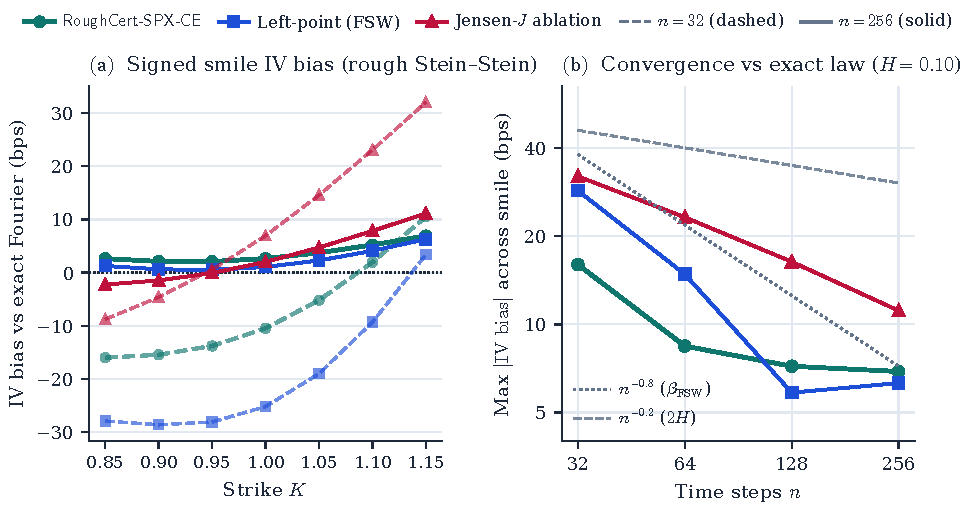
\includegraphics[width=\textwidth]{figures/fig_e1_exact_rss.pdf}
  \caption{Exact-law validation on correlated rough Stein--Stein ($H=0.10$, $T=0.5$, $\rho=-0.7$). (a) IV bias across strikes at $n=32$ and $n=256$ against the $M=\EOneRSSMop$ Fourier reference. (b) Maximum smile IV bias across dyadic levels for \RCCE{}, left-point and the Jensen-$J$ ablation, with reference slopes.}
  \label{fig:e1_rss}
\end{figure}

Three observations follow.
\begin{itemize}
  \item \emph{Containment.} All three envelopes contain the reference price at all seven strikes; the \RCCE{} and left-point envelopes carry \EOneRSSCeDiag{} diagnostic flags. This is consistent with Theorem~\ref{thm:bridge_envelope} on a rough correlated benchmark whose reference has no Monte Carlo error.
  \item \emph{Variance-channel projection reduces coarse-grid error.} At $n=32$, \RCCE{} lowers the maximum smile IV bias from $\EOneRSSLPMaxLow\bps$ (left-point) to $\EOneRSSCeMaxLow\bps$, a reduction by a factor of at least $\EOneRSSCeGainLow$, and the two estimators agree at $n=256$ ($\EOneRSSCeMaxFine\bps$ and $\EOneRSSLPMaxFine\bps$).
  \item \emph{Jensen-$J$ smoothing is worse at every level.} The ablation has the largest bias on every grid ($\EOneRSSJenMaxLow\bps$ at $n=32$ and $\EOneRSSJenMaxFine\bps$ at $n=256$, at least $\EOneRSSJenOverLPFine$ times the left-point value) and $\EOneRSSJenDiag$ diagnostic flags, consistent with the correlation attenuation of Proposition~\ref{prop:jensen_pitfall}(ii).
\end{itemize}

\subsection{Experiment E2: testing the full-determinism hypothesis}
\label{sec:e2}

We compute \emph{Arb-certified} \RCDet{} ATM brackets on a $\ETwoGridNH\times\ETwoGridNEta$ grid of $H\in\{0.05,\allowbreak 0.07,\allowbreak 0.10,\allowbreak 0.15,\allowbreak 0.20,\allowbreak 0.30,\allowbreak 0.40,\allowbreak 0.45\}$ and dimensionless vol-of-vol $\eta_{\mathrm{eff}}=\eta T^H\in[0.02,1.50]$ ($T=0.25$, $\xi_0=0.04$), and locate the $10\bps$, $25\bps$ and $50\bps$ boundaries by $\ETwoBisectSteps$-step bisection (resolution $\ETwoBisectTol$; each boundary is the last certified point) for $\rho=0$ (two-moment bound, Proposition~\ref{prop:twomoment}), $\rho=-0.5$ and $\rho=-0.9$ (Theorem~\ref{thm:put_lipschitz}). Figure~\ref{fig:e2_phase} shows the certifiability landscape, and Table~\ref{tab:e2_spotlights} pairs \RCDet{} with \RCBridge{} in seven spotlight regimes S1--S7.

\begin{figure}[t]
  \centering
  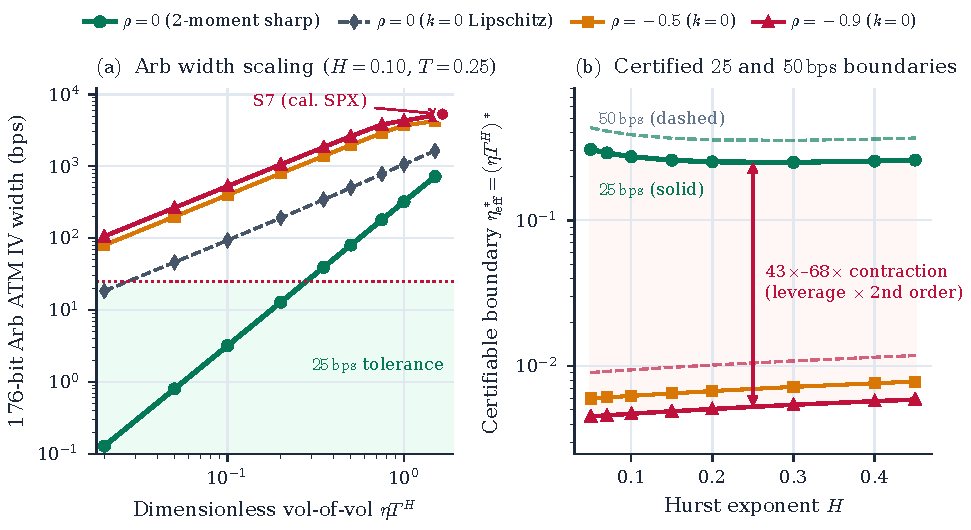
\includegraphics[width=\textwidth]{figures/fig_e2_phase_map.pdf}
  \caption{Deterministic certifiability phase map (ATM, $T=0.25$, $\xi_0=0.04$). (a) Certified IV width against $\eta T^H$ for $\rho=0$ (Proposition~\ref{prop:twomoment}), $\rho=-0.5$ and $\rho=-0.9$ (Theorem~\ref{thm:put_lipschitz}). (b) Certified $25\bps$ and $50\bps$ boundaries across $H$.}
  \label{fig:e2_phase}
\end{figure}

\begin{table}[t]
\centering
\caption{Spotlight comparison of \ArbBits-bit Arb \RCDet{} and \RCBridge{} ATM implied-volatility widths ($\xi_0=0.04$, $25\bps$ desk gate).}
\label{tab:e2_spotlights}
\footnotesize
\setlength{\tabcolsep}{3.6pt}
\begin{tabular}{@{}lrrrrrrlll@{}}
\toprule
Spotlight & $H$ & $T$ & $\eta$ & $\rho$ & Det width & Bridge width & Bridge & Arb & Gate \\
regime & & (yr) & & & (bps, Arb) & (bps, stat.) & status & cont.? & choice \\
\midrule
S1: Mild, $\rho=0$ & 0.30 & 0.10 & 0.30 & $0.0$ & 8.72 & 0.02 & Asymp.-env. & Yes & Tier~1 (Arb) \\
S2: Rough, $\rho=0$ & 0.10 & 0.25 & 0.20 & $0.0$ & 9.21 & 0.03 & Asymp.-env. & Yes & Tier~1 (Arb) \\
S3: 1-day, corr. & 0.30 & $1/252$ & 0.03 & $-0.7$ & 22.54 & 0.12 & Asymp.-env. & Yes & Tier~1 (Arb) \\
S4: Rough, mild $\eta$ & 0.10 & 0.25 & 0.10 & $-0.7$ & 413.0 & 0.44 & Asymp.-env. & Yes & Tier~3 (Bridge) \\
S5: Rough, mod.\ $\eta$ & 0.10 & 0.25 & 0.50 & $-0.7$ & 2044.3 & 5.59 & Asymp.-env. & Yes & Tier~3 (Bridge) \\
S6: Cal.\ $\eta$, $\rho=0$ & 0.10 & 0.25 & 1.90 & $0.0$ & 823.3 & 9.64 & Asymp.-env. & Yes & Tier~3 (Bridge) \\
S7: Cal.\ SPX full & 0.10 & 0.25 & 1.90 & $-0.9$ & 5301.8 & 18.43 & Asymp.-env. & Yes & Tier~3 (Bridge) \\
\bottomrule
\end{tabular}
\par\smallskip
\parbox{\linewidth}{\footnotesize\emph{Notes.} Det: deterministic Arb-certified ATM IV width (Proposition~\ref{prop:twomoment} for $\rho=0$, Theorem~\ref{thm:put_lipschitz} for $\rho<0$). Bridge: asymptotic-envelope statistical(0.95) width (Theorem~\ref{thm:bridge_envelope}; levels $32$--$256$, $32{,}768$ RQMC paths). The two widths carry different guarantees. Arb cont.: the Arb bracket contains the Bridge midpoint.}
\end{table}
%

Experiment~E2 settles the hypothesis quantitatively.
\begin{enumerate}[1.]
  \item \emph{Zero leverage.} The two-moment bound is of second order and certifies ATM IV to $25\bps$ up to $\eta T^H\in[\ETwoRhoZeroMin,\ETwoRhoZeroMax]$ across $H\in[0.05,0.45]$, which is $\ETwoSecondOrderMin$--$\ETwoSecondOrderMax$ times further than the first-order bracket reaches at $\rho=0$ ($\eta T^H\in[\ETwoRhoZeroFirstMin,\ETwoRhoZeroFirstMax]$). Spotlights S1 ($\ETwoSOneDet\bps$) and S2 ($\ETwoSTwoDet\bps$, $H=0.10$) pass the desk gate in Arb alone.
  \item \emph{Leverage.} At $\rho=-0.9$ the $25\bps$ boundary drops to $\eta T^H\in[\ETwoRhoNineMin,\ETwoRhoNineMax]$, a contraction by a factor of $\ETwoCollapseMin$--$\ETwoCollapseMax$. It factors into a leverage factor of $\ETwoLeverageMin$--$\ETwoLeverageMax$, obtained with the same first-order bracket at $\rho=0$ and $\rho=-0.9$, and the second-order factor above, which is lost because the two-moment bound exists only at $\rho=0$ (Supplementary Table~S2). The leverage factor is almost constant in $H$ because both first-order brackets scale with the same residual $E_J$; they differ through the coefficients of Theorem~\ref{thm:put_lipschitz} and through the concavity cap $C(1)\le C_\BS(1,1,\E[I_T])$ that tightens the $\rho=0$ bracket from above. Only very short or very mild regimes such as S3 (one-day maturity, $\ETwoSThreeDet\bps$) pass deterministically.
  \item \emph{Calibrated SPX parameters need Tier~3.} At S7 ($H=0.10$, $T=0.25$, $\eta=1.9$, $\rho=-0.9$), \RCDet{} gives a deterministic envelope of width $\ETwoSSevenDet\bps$, which contains the Bridge midpoint as in all seven spotlights. The \RCBridge{} envelope is $\ETwoSSevenBridge\bps$ wide, narrower by a factor of at least $\ETwoSSevenRatio$, but it carries the \emph{asymptotic-envelope statistical(0.95)} label rather than a deterministic guarantee; all seven spotlights reach that status, with widths down to $\ETwoSFourBridge\bps$ at S4.
\end{enumerate}
A code-disjoint recomputation with the exact formulas (checks I1--I2, Supplementary Table~S5) confirms that every stored Arb bracket contains the exact-formula bracket and that the exact ATM width at the stored $25\bps$ boundary points for $H=0.10$ and $H=0.30$ is at most $\IndepETwoMaxExactWidth\bps$. The Arb brackets are wider than the exact-formula brackets by $\ETwoArbOverheadMin$--$\ETwoArbOverheadMax\%$, mostly in the $\rho=0$ spotlights, where the box enclosure of $\Var(I_T)$ enters the two-moment bound.

\FloatBarrier
